\ifnum \Solutions=0
\newpage 
\fi
\ifnum \Version=1
    \question[5] Consider the non-linear system below.  
    \begin{align*}
        \dxdt &= y(x+y-6) , \qquad \dydt = x(2x+y-8)
    \end{align*}
    \begin{parts}
        \part Determine the locations of the critical points. 
        \ifnum \Solutions=1 {\color{DarkBlue} \\[12pt] 
        Setting both $x'=0$ and $y'=0$, we obtain four critical points as follows. $x'=0$ implies $y=0$ or $x+y-6=0$. 
            \begin{itemize}
                \item If $y=0$, then for $y'=0$ we need either $x=0$ or $2x+y-8=0$. 
                \begin{itemize}
                    \item If $y=0$ and $x=0$, one critical point is at $(0,0)$. 
                    \item If $y=0$ and $2x+y-8=0$, one critical point is at $(4,0)$. 
                \end{itemize}
                \item If $x+y-6=0$, then for $y'=0$ we need either $x=0$ or $2x+y-8=0$. 
                \begin{itemize}
                    \item If $x+y-6=0$ and $x=0$, one critical point is at $(0,6)$. 
                    \item If $x+y-6=0$ and $2x+y-8=0$, then solving this system of equations yields a critical point at $(2,4)$. 
                \end{itemize}                
            \end{itemize}
            The four critical points are located at $(0,0)$, $(4,0)$, $(0,6)$, $(2,4)$. 
            } 
        \else 
        \vfill
        \fi
        \part Sketch the nullclines of the system on the axes below. Clearly indicate the critical points that you found in part (a). 
        \ifnum \Solutions=1 {\color{DarkBlue} \\[12pt] 
        Green lines are the $x-$nullclines, red lines are the $y-$nullclines.
        \begin{center}
        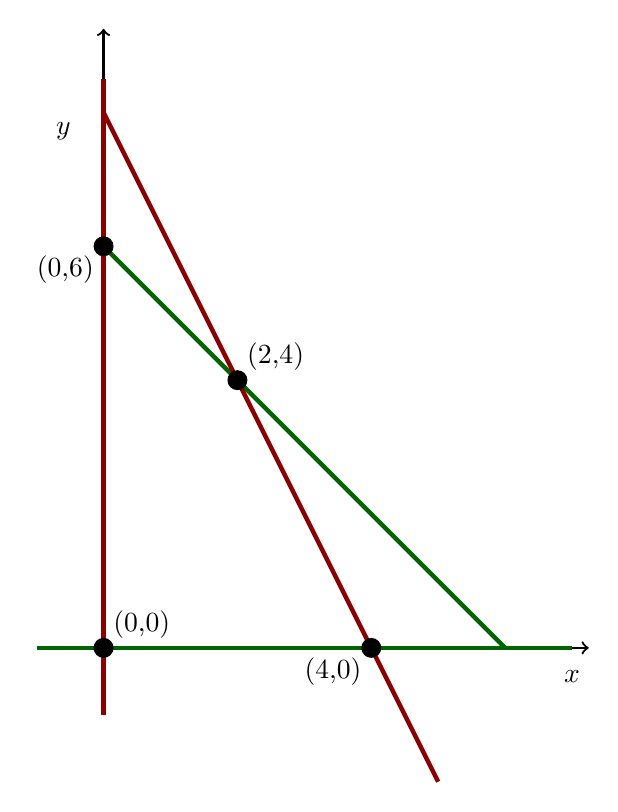
\begin{tikzpicture}[scale=0.85]
        \draw[thick, ->] (-1, 0) -- (7.25, 0);
        \draw[thick, ->] (0, -1) -- (0, 9.25);
        \node[overlay, below] at (7, -0.2) {$x$};
        \node[overlay, below] at (-0.6, 8) {$y$};   
        \draw[ultra thick,DarkGreen, -] (-1, 0) -- (7, 0);        
        \draw[ultra thick,DarkGreen, -] (0,6) -- (6, 0);   
        \draw[ultra thick,DarkRed, -] (0, 8) -- (5, -2);        
        \draw[ultra thick,DarkRed, -] (0, -1) -- (0, 8.5);      
        \filldraw[black] (0,0) circle (4pt) node[anchor=south west]{(0,0)};
        \filldraw[black] (0,6) circle (4pt) node[anchor=north east]{(0,6)};
        \filldraw[black] (2,4) circle (4pt) node[anchor=south west]{(2,4)};
        \filldraw[black] (4,0) circle (4pt) node[anchor=north east]{(4,0)};
        \end{tikzpicture}
        \end{center}            
        } 
        \else 
        \begin{center}
        \begin{tikzpicture}[scale=0.55]
        \draw[very thick, ->] (-6, 0) -- (6.25, 0);
        \draw[very thick, ->] (0, -6) -- (0, 6.25);
        \node[overlay, below] at (6, -0.2) {$x$};
        \node[overlay, below] at (-0.6, 6) {$y$};        
        \end{tikzpicture}
        \end{center}    
    \fi
    \end{parts}
\fi 





\ifnum \Version=2
    \question[6] Consider the non-linear system below.  
    \begin{align*}
        \dxdt &= (x-1)(y-5) , \qquad \dydt = y-x^2-1
    \end{align*}
    \begin{parts}
        \part Determine the locations of the critical points. 
        \ifnum \Solutions=1 {\color{DarkBlue} \\[12pt] 
        For a point to be a critical point, we need $x' = y' = 0$. If $x'$ is zero, then either $x=1$ or $y=5$. 
        \begin{itemize}
            \item When $x=1$, for $y'=0$ we need 
            \begin{align}
                y'&=0 = y - x^2 - 1 \quad \Rightarrow \quad y = 1^2+1 = 2
            \end{align}
            There is a critical point at $(1,2)$. 
            \item When $y=5$, for $y'=0$ we need 
            \begin{align}
                y'&=0 = y - x^2 - 1 \quad \Rightarrow \quad x^2 = 5 - 1 \quad \Rightarrow \quad x = \pm 2
            \end{align}
            There are critical points at $(\pm 2, 5)$.             
        \end{itemize}
            } 
        \else 
        \vfill
        \fi
        \part Sketch the nullclines of the system on the axes below. Clearly indicate the critical points that you found in part (a). 
        \ifnum \Solutions=1 {\color{DarkBlue} \\[12pt] 
        The curves are shown below. The green lines are the x nullclines, and the red curve is the y nullcline. There are exactly three critical points. 
            \begin{center}
            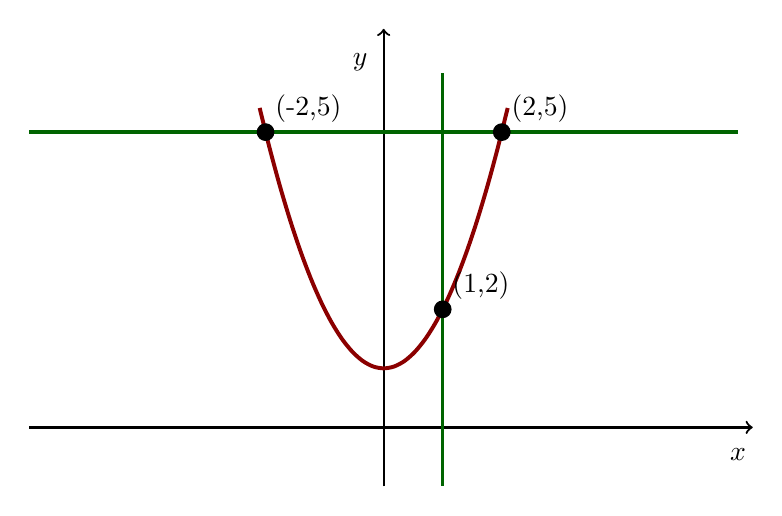
\begin{tikzpicture}[scale=0.75]
            \draw[thick, ->] (-6, 0) -- (6.25, 0);
            \draw[thick, ->] (0, -1) -- (0, 6.75);
            \node[overlay, below] at (6, -0.2) {$x$};
            \node[overlay, below] at (-0.4, 6.5) {$y$};   
            \draw[very thick,DarkGreen, -] (1, 6) -- (1, -1);        
            \draw[very thick,DarkGreen, -] (-6, 5) -- (6, 5);   
            \draw[DarkRed, line width = 0.50mm]   plot[smooth,domain=-2.1:2.1] (\x, {\x*\x+1});
            \filldraw[black] (2,5) circle (4pt) node[anchor=south west]{(2,5)};
            \filldraw[black] (-2,5) circle (4pt) node[anchor=south west]{(-2,5)};
            \filldraw[black] (1,2) circle (4pt) node[anchor=south west]{(1,2)};
            \end{tikzpicture}
            \end{center}               
        } 
        \else 
        \begin{center}
        \begin{tikzpicture}[scale=0.55]
        \draw[very thick, ->] (-6, 0) -- (6.25, 0);
        \draw[very thick, ->] (0, -6) -- (0, 6.25);
        \node[overlay, below] at (6, -0.2) {$x$};
        \node[overlay, below] at (-0.6, 6) {$y$};        
        \end{tikzpicture}
        \end{center}    
    \fi
    \end{parts}
\fi 




\ifnum \Version=3
    \question[6] Consider the non-linear system below.  
    \begin{align*}
        \dxdt &= (x-1)(y-2) , \qquad \dydt = y^2-x
    \end{align*}
    \begin{parts}
        \part Determine the locations of the critical points. 
        \ifnum \Solutions=1 {\color{DarkBlue} \\[12pt] 
        For a point to be a critical point, we need $x' = y' = 0$. If $x'$ is zero, then either $x=1$ or $y=2$. 
        \begin{itemize}
            \item When $x=1$, for $y'=0$ we need 
            \begin{align}
                y'&=0 = y^2 - x \quad \Rightarrow \quad y = \pm 1
            \end{align}
            There are critical points at $(1,\pm 1)$. 
            \item When $y=2$, for $y'=0$ we need 
            \begin{align}
                y'&=0 = y^2 - x  \quad \Rightarrow \quad x = 4 
            \end{align}
            There is a critical point at $(4, 2)$.             
        \end{itemize}
            } 
        \else 
        \vfill
        \fi
        \part Sketch the nullclines of the system on the axes below. Clearly indicate the critical points that you found in part (a). 
        \ifnum \Solutions=1 {\color{DarkBlue} \\[12pt] 
        The curves are shown below. The green lines are the x nullclines, and the red curve is the y nullcline. There are exactly three critical points. 
            \begin{center}
            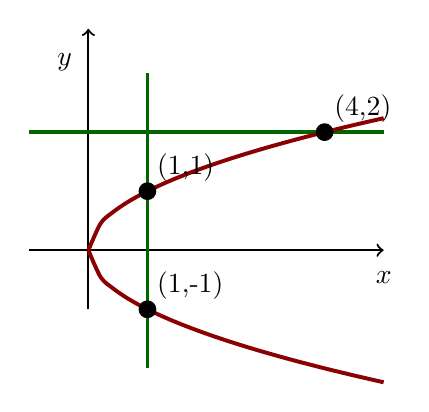
\begin{tikzpicture}[scale=0.75]
            \draw[thick, ->] (-1, 0) -- (5, 0);
            \draw[thick, ->] (0, -1) -- (0, 3.75);
            \node[overlay, below] at (5, -0.2) {$x$};
            \node[overlay, below] at (-0.4, 3.5) {$y$};   
            \draw[very thick,DarkGreen, -] (1, 3) -- (1, -2);        
            \draw[very thick,DarkGreen, -] (-1, 2) -- (5, 2);   
            \draw[DarkRed, line width = 0.50mm]   plot[smooth,domain=0:5] (\x, {\x^(1/2))} );
            \draw[DarkRed, line width = 0.50mm]   plot[smooth,domain=0:5] (\x, {-\x^(1/2))} );
            \filldraw[black] (4,2) circle (4pt) node[anchor=south west]{(4,2)};
            \filldraw[black] (1,1) circle (4pt) node[anchor=south west]{(1,1)};
            \filldraw[black] (1,-1) circle (4pt) node[anchor=south west]{(1,-1)};
            \end{tikzpicture}
            \end{center}               
        } 
        \else 
        \begin{center}
        \begin{tikzpicture}[scale=0.55]
        \draw[very thick, ->] (-6, 0) -- (6.25, 0);
        \draw[very thick, ->] (0, -6) -- (0, 6.25);
        \node[overlay, below] at (6, -0.2) {$x$};
        \node[overlay, below] at (-0.6, 6) {$y$};        
        \end{tikzpicture}
        \end{center}    
    \fi
    \end{parts}
\fi 


\ifnum \Version=6
    \question[4] Consider the non-linear system below.  
    \begin{align*}
        \dxdt &= (x-2)(y-1) , \qquad \dydt = 2y^2-x
    \end{align*}
    \begin{parts}
        \part Determine the locations of the critical points. 
        \ifnum \Solutions=1 {\color{DarkBlue} \\[12pt] 
        For a point to be a critical point, we need $x' = y' = 0$. If $x'$ is zero, then either $x=2$ or $y=1$. 
        \begin{itemize}
            \item When $x=2$, for $y'=0$ we need 
            \begin{align}
                y'&=0 = 2y^2 - x \quad \Rightarrow \quad y = \pm 1
            \end{align}
            There are critical points at $(2,\pm 1)$. 
            \item When $y=1$, for $y'=0$ we need 
            \begin{align}
                y'&=0 = 2y^2 - x  \quad \Rightarrow \quad x = 2
            \end{align}
            There is a critical point at $(2,1)$, which we already had.          
        \end{itemize}
            } 
        \else 
        \vfill
        \fi
        \part Sketch the nullclines of the system on the axes below. Clearly indicate the critical points that you found in part (a). 
        \ifnum \Solutions=1 {\color{DarkBlue} \\[12pt] 
        The curves are shown below. The green lines are the x nullclines, and the red curve is the y nullcline. There are exactly three critical points. 
            \begin{center}
            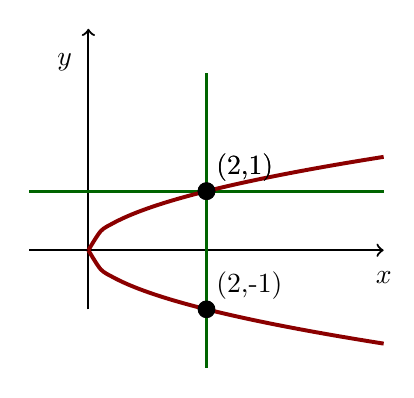
\begin{tikzpicture}[scale=0.75]
            \draw[thick, ->] (-1, 0) -- (5, 0);
            \draw[thick, ->] (0, -1) -- (0, 3.75);
            \node[overlay, below] at (5, -0.2) {$x$};
            \node[overlay, below] at (-0.4, 3.5) {$y$};   
            \draw[very thick,DarkGreen, -] (2, 3) -- (2, -2);        
            \draw[very thick,DarkGreen, -] (-1, 1) -- (5, 1);   
            \draw[DarkRed, line width = 0.50mm]   plot[smooth,domain=0:5] (\x, {(\x/2)^(1/2))} );
            \draw[DarkRed, line width = 0.50mm]   plot[smooth,domain=0:5] (\x, {-(\x/2)^(1/2))} );
            \filldraw[black] (2,1) circle (4pt) node[anchor=south west]{(2,1)};
            \filldraw[black] (2,1) circle (4pt) node[anchor=south west]{(2,1)};
            \filldraw[black] (2,-1) circle (4pt) node[anchor=south west]{(2,-1)};
            \end{tikzpicture}
            \end{center}               
        } 
        \else 
        \begin{center}
        \begin{tikzpicture}[scale=0.55]
        \draw[very thick, ->] (-6, 0) -- (6.25, 0);
        \draw[very thick, ->] (0, -6) -- (0, 6.25);
        \node[overlay, below] at (6, -0.2) {$x$};
        \node[overlay, below] at (-0.6, 6) {$y$};        
        \end{tikzpicture}
        \end{center}    
    \fi
    \end{parts}
\fi 


\ifnum \Version=7
    \question[4] Consider the non-linear system below.  
    \begin{align*}
        \dxdt &= (x-1)(y-5) , \qquad \dydt = y-x^2-1
    \end{align*}
    \begin{parts}
        \part Determine the locations of the critical points. 
        \ifnum \Solutions=1 {\color{DarkBlue} \\[12pt] 
        For a point to be a critical point, we need $x' = y' = 0$. If $x'$ is zero, then either $x=1$ or $y=5$. 
        \begin{itemize}
            \item When $x=1$, for $y'=0$ we need 
            \begin{align}
                y'&=0 = y - x^2 - 1 \quad \Rightarrow \quad y = 1^2+1 = 2
            \end{align}
            There is a critical point at $(1,2)$. 
            \item When $y=5$, for $y'=0$ we need 
            \begin{align}
                y'&=0 = y - x^2 - 1 \quad \Rightarrow \quad x^2 = 5 - 1 \quad \Rightarrow \quad x = \pm 2
            \end{align}
            There are critical points at $(\pm 2, 5)$.             
        \end{itemize}
            } 
        \else 
        \vfill
        \fi
        \part Sketch the nullclines of the system on the axes below. Clearly indicate the critical points that you found in part (a). 
        \ifnum \Solutions=1 {\color{DarkBlue} \\[12pt] 
        The curves are shown below. The green lines are the x nullclines, and the red curve is the y nullcline. There are exactly three critical points. 
            \begin{center}
            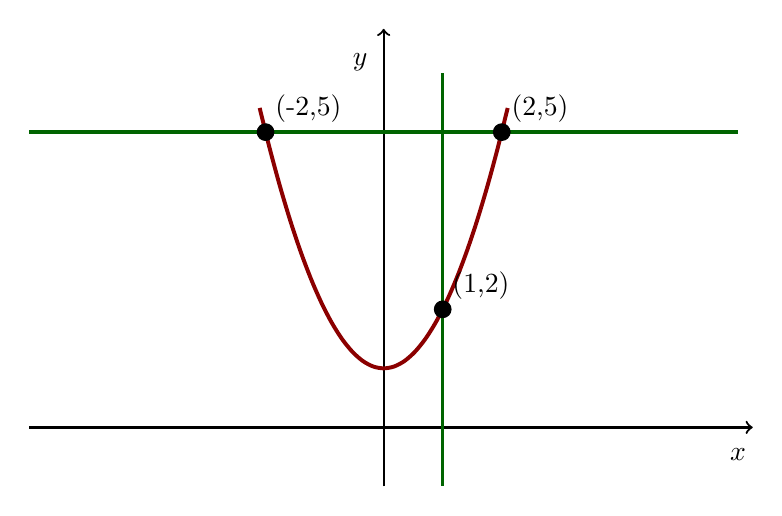
\begin{tikzpicture}[scale=0.75]
            \draw[thick, ->] (-6, 0) -- (6.25, 0);
            \draw[thick, ->] (0, -1) -- (0, 6.75);
            \node[overlay, below] at (6, -0.2) {$x$};
            \node[overlay, below] at (-0.4, 6.5) {$y$};   
            \draw[very thick,DarkGreen, -] (1, 6) -- (1, -1);        
            \draw[very thick,DarkGreen, -] (-6, 5) -- (6, 5);   
            \draw[DarkRed, line width = 0.50mm]   plot[smooth,domain=-2.1:2.1] (\x, {\x*\x+1});
            \filldraw[black] (2,5) circle (4pt) node[anchor=south west]{(2,5)};
            \filldraw[black] (-2,5) circle (4pt) node[anchor=south west]{(-2,5)};
            \filldraw[black] (1,2) circle (4pt) node[anchor=south west]{(1,2)};
            \end{tikzpicture}
            \end{center}               
        } 
        \else 
        \begin{center}
        \begin{tikzpicture}[scale=0.55]
        \draw[very thick, ->] (-6, 0) -- (6.25, 0);
        \draw[very thick, ->] (0, -6) -- (0, 6.25);
        \node[overlay, below] at (6, -0.2) {$x$};
        \node[overlay, below] at (-0.6, 6) {$y$};        
        \end{tikzpicture}
        \end{center}    
    \fi
    \end{parts}
\fi 
